\section{Pipelining}
	\subsection{RISC vs. CISC}
		RISC(Reduced Instruction Set Computer)(x86) \newline
		CISC(Complex Instruction Set Computer)(RISC-V)
		\subsubsection{CISC}
			Vorteile: \newline
			\begin{itemize}
				\item Geringe Speicherdichte für Programmcode erforderlich. Mit weniger Assemblerfunktionen kann man mehr Funktionalität erreichen
				\item Einfacher, kompakter Code
			\end{itemize}
			Nachteile: \newline
			\begin{itemize}
				\item sehr große und undurchschaubare Befehlssätze
				\item nur kleiner Teil der Befehlssätze wurde tatsächlich verwendet
			\end{itemize}
		\subsubsection{RISC}	
			Merkmale: \newline
			\begin{itemize}
				\item Kleine, einheitliche Machinenbefehlssätze
				\item Adressberechnung durch explizite Befehle durch führen
				\item Load-Store-Architektur: Alle Operanden liegen in Registern, Zugriff auf Speicheradressen mittels expliziter Lade- bzw. Speicherbefehle
				\item Große Anzahl universell nutzbarer Register
				\item Festverdrahtete Leitwerke: kein Mikroprogramm; jeder RISC-Befehl wird direkt in binäres Befehlsmuster dekodiert
				\item Konsequentes Ausnutzen von Pipelining
			\end{itemize}
	\subsection{Grundlagen}
		Das grundlegende Prinzip von Pipelining (Fließbandverarbeitung) ist, dass verschiedene Phasen verschiedener, unabhängiger Befehle gleichzeitig durchlaufen werden. Dies kann man auch als pseudoparallele Verarbeitung bezeichnen. \newline \newline
		RISC-V-Befehlszyklus: \newline
		\begin{itemize}
			\item BH: Befehl holen
			\item BD/OH: Befehl dekodieren und Operanden holen
			\item BA: Befehl ausführen
			\item MEM: Speicherzugriff
			\item RE: Rückschreibephase
		\end{itemize}
		Zwischen die einzelnen Stufen werden Register eingefügt. Dies ist nötig, damit die Werte unterschiedlicher Befehle voneinander entkoppelt werden und sich nicht gegenseitig beeinflussen. Hätte man keine Zwischenregister, würde das Ergebnis von Phase A in Phase B "reinlaufen", während Phase B noch nicht mit der vorherigen Instruktion fertig ist. \newline \newline
		Die Einführung der Register sorgt außerdem dafür, dass es nicht einen langen Datenpfad, sondern mehrere kürzere Datenpfade gibt. Ein Datenpfad sind die Leitungen und logischen Gatter, die zwischen zwei Speicherzellen/Registern durchlaufen werden müssen. 
		Dadurch wird der kritische Pfad (= längster Datenpfad) ebenfalls kürzer, wodurch der Takt angehoben werden kann, da weniger Logik pro Takt ausgeführt werden muss. \newline \newline
		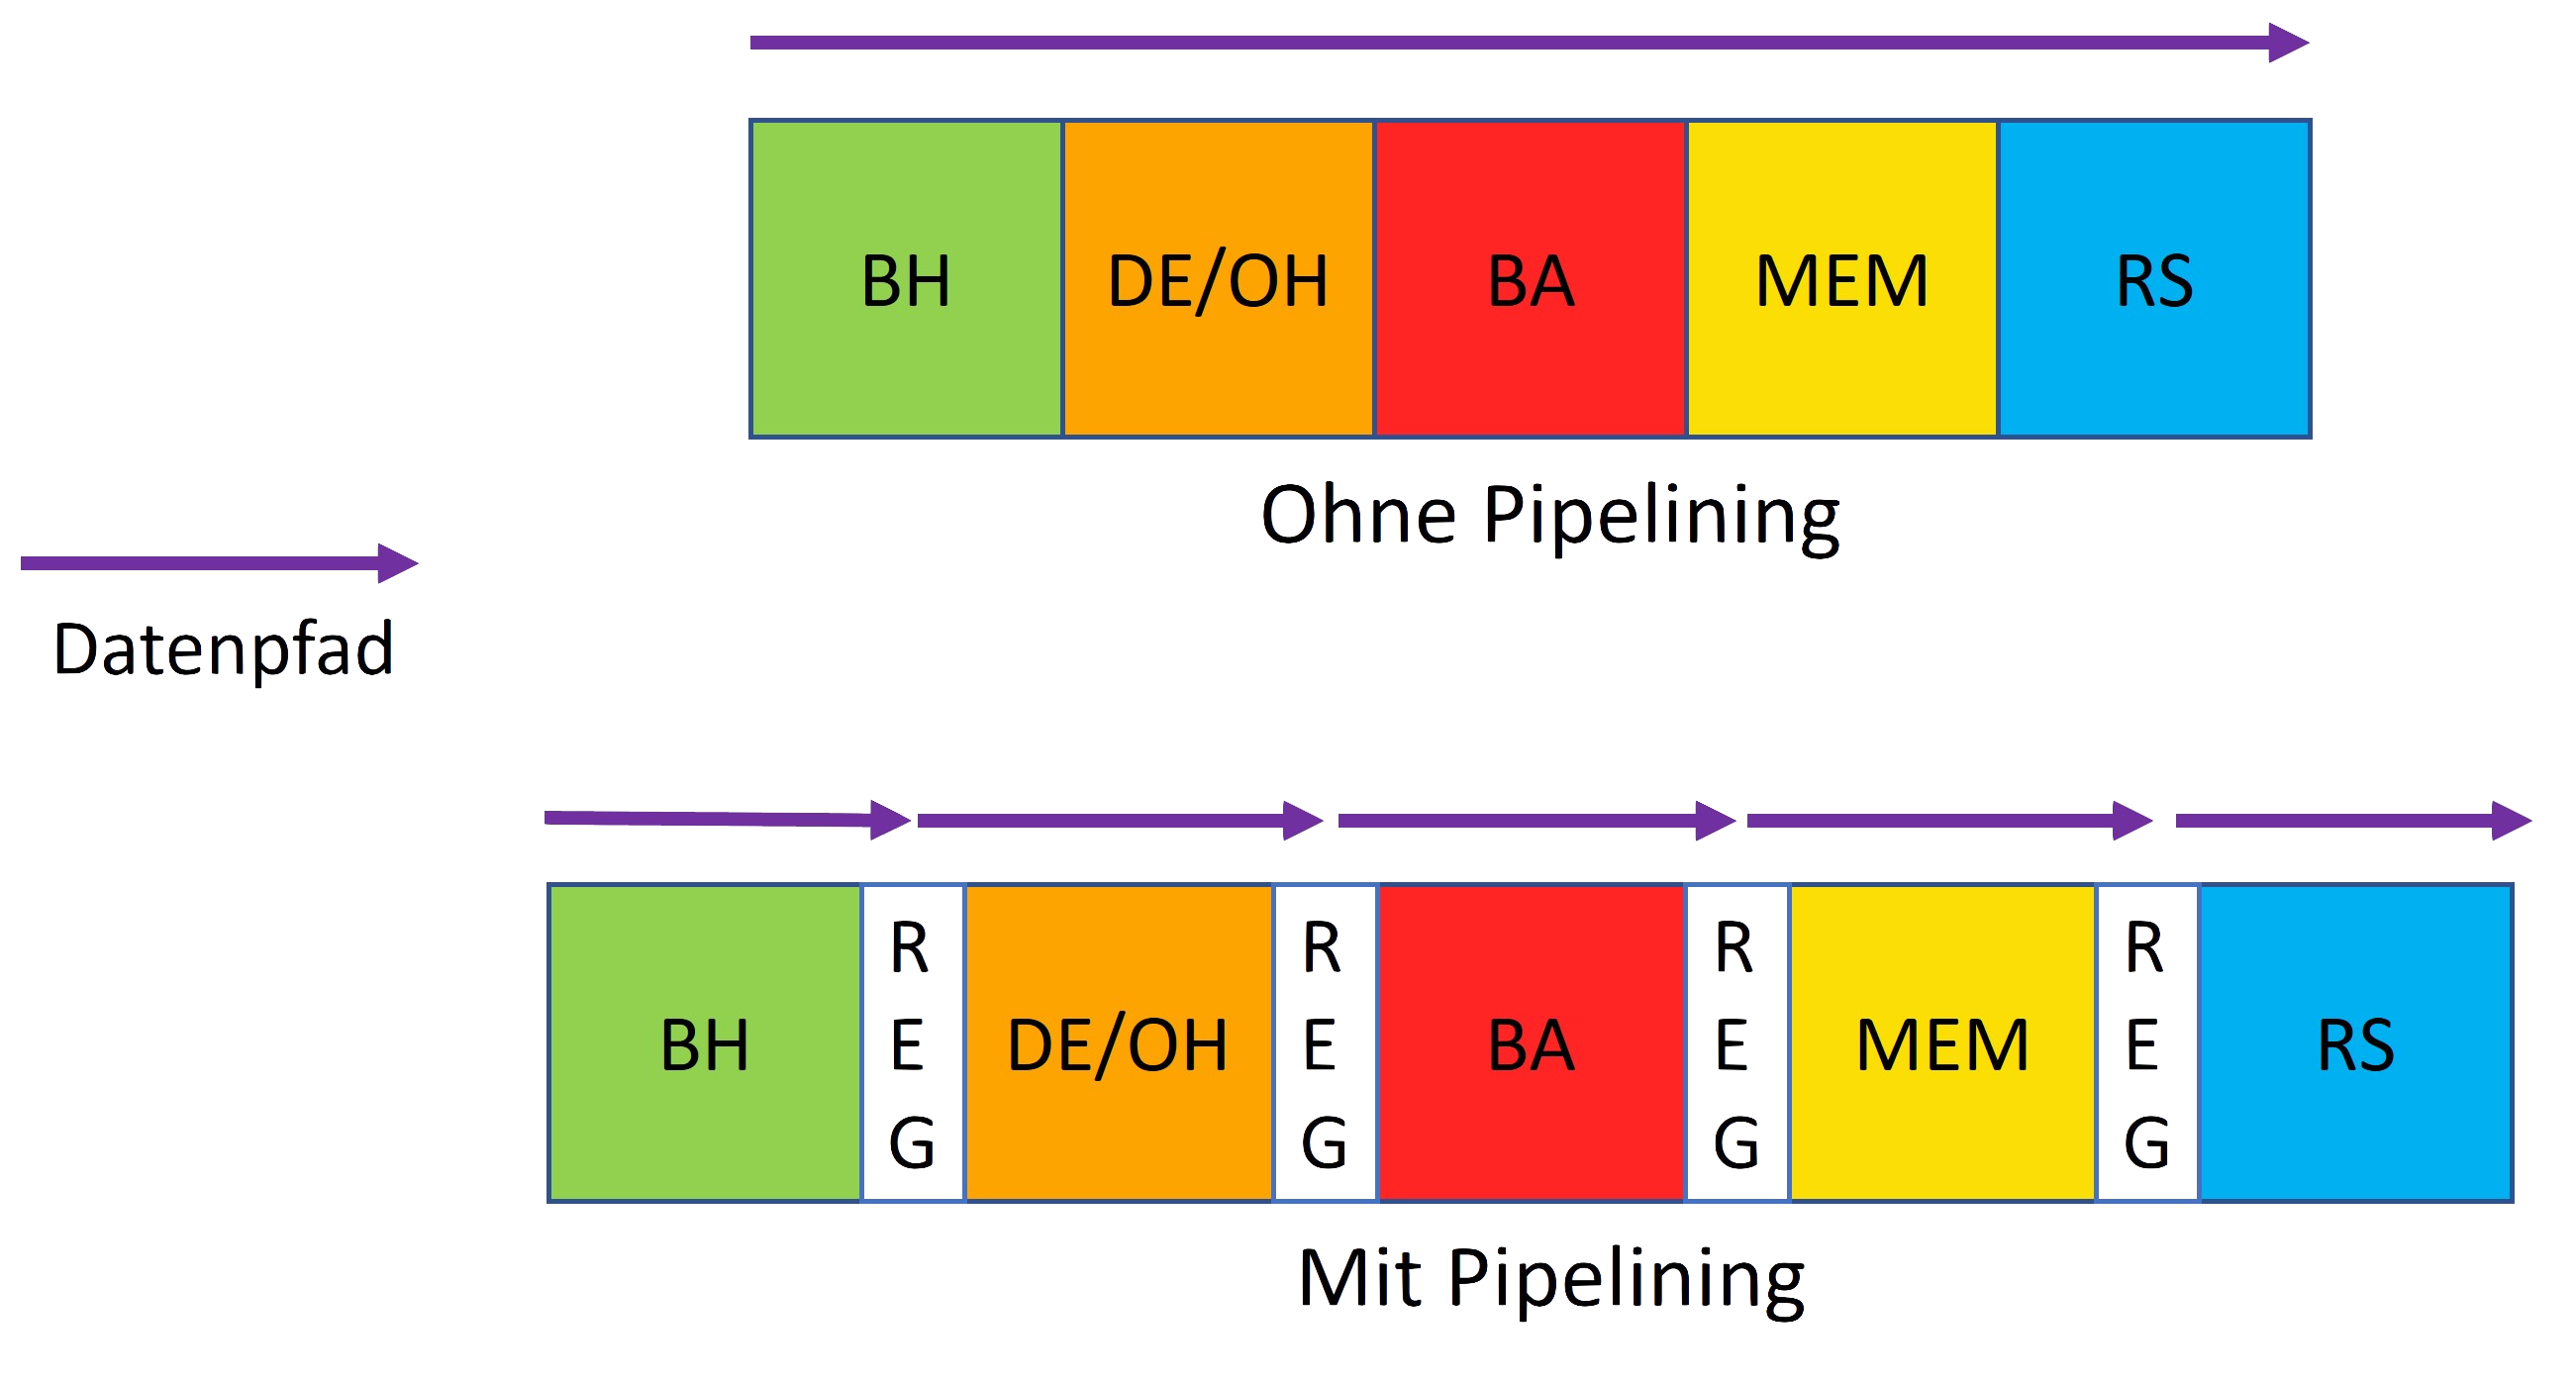
\includegraphics[scale=0.6]{Datenpfade_mit_und_ohne_Pipeline.png}
	\subsection{Speedup}
		Ausführung ohne Pipelining:
		$$
			T_{seq}=(\displaystyle\sum^k_{i-1}\tau_i)\cdot n
		$$
		Ausführung mit Pipelining:
		$$
			T_{par}=k\cdot\tau_{max}+(k-1)\cdot d_{Reg}+(n-1)\cdot(\tau_{max}+d_{Reg})
		$$
		$\tau_{max}=\texttt{max}_{1\leq i\leq k}\{\tau_i\}$ steht für die Ausführungszeit der langsamsten Stufe\newline
		$k\cdot\tau_{max}+(k-1)\cdot d_{Reg}$: Der erste Befehl läuft durch alle $k$ Pipelinestufen \newline \newline
		\textbf{Speedup allgemein}:
		$$
			S=\frac{T_{seq}}{T_{par}}=\frac{\texttt{sequentielle Ausführung}}{\texttt{parallele Ausführung}}
		$$
	\subsection{Hazards}
		\subsubsection{Datenhazards}
			Entstehen durch Datenabhänigkeit. Dabei wird das Ergebnis der vorherigen Instruktionen von der aktuelle Instruktion benötigt, ist aber noch nicht verfügbar
		\subsubsection{Steuerungshazards}
			Treten unter Umständen bei Befehlen auf, die den Befehlszähler verändern, wie bspw. bedingte Sprünge. Es gelangen Befehle in der Pipeline, die anschließend wieder verworfen werden müssen, weil an eine andere Stelle gesprungen wird
		\subsubsection{Strukturhazards}
			Entstehen, wenn gleichzeitig auf eine Hardwarekomponente (z.B. gleiche Recheneinheit) zugegriffen wird